\section{Porous medium properties}

We have considered the properties of fluid (section \ref{sec:fluid_properties}) and solid phases (section \ref{sec:m_properties}), respectively. Many of the properties of a porous medium can be determined based on the assumption of the local thermodynamic equillibrium allowing a superposition of phase related characteristics - except of the hydraulic properties for multiphase flow, which are discussed in this section in more detail. We restart with the different definitions of saturation.

\subsection{Saturation}

Saturation of a fluid phase $\gamma$ is defined as the volumetric fraction $\epsilon^\gamma$ related to the sum of all fluid phases volumetric fractions.
%
\begin{eqnarray}
S^\gamma =
\frac{\epsilon^\gamma}{\sum_{\gamma}\epsilon^\gamma}
\end{eqnarray}

The sum of saturations of all fluid phases must be equal to unity (section \ref{sec:mixtures}).
%
Effective saturation is defined as \cite{BroCor:64}
%
\begin{eqnarray}
S_{\mbox{\small eff}}^\gamma =
\frac{S^\gamma-S_r^\gamma}{1-S_r^\gamma}
\end{eqnarray}

Moisture content (volumetric water content) is defined as the
product of porosity and saturation.
\begin{eqnarray}
\theta^\gamma = n S^\gamma
\end{eqnarray}

Gravimetric water content is defined as
\begin{eqnarray}
\omega^\gamma
=
n S^\gamma
\frac{\rho_d^s}{\rho^\gamma}
\end{eqnarray}

Applying the chain rule, we can express saturation changes in
following way.
\begin{eqnarray}
dS^\gamma =
\frac{dS^\gamma}{dp^\gamma} dp^\gamma
\end{eqnarray}

The capillary pressure-saturation functions as well as the relations between relative permeability and saturation are substantial constitutive equations required for multiphase flow. Within this context, usually algebraic expressions are fit to the corresponding experimentally observed curves. Among the widely-used of these algebraic expressions are the Brooks-Corey \cite{BC:1964} and van Genuchten \cite{Van:80} relations. If both are realized within the scientific software code developed by the authors, the numerical results presented in this paper are based on Brooks-Corey's approach.

%---
\subsection{Capillary pressure and relative permeability}
\index{quantity - pressure capillary}

As a consequence of interfacial tension a discontinuity in fluid
pressure exists across the interface that separates two immiscible
fluids. The partial pressure difference between two phases is
denoted as capillary pressure, which is a function of saturation.
%
\begin{eqnarray}
p_c^{\alpha\beta} = p^\beta -
p^\alpha = f(S^\alpha)
\end{eqnarray}

In general, capillary pressure is the difference between partial
pressures of non-wetting and wetting phases.
\begin{eqnarray}
p_c = p^{nw} - p^w =
f(S^w) 
\label{eqn:capillary_pressure}
\end{eqnarray}

Capillary pressure is always positive: $p_c>0 ,
\forall S$. It is often assumed that air is at a constant
atmospheric pressure taken as zero $p^g=0$. This means,
the macroscopic pressure of water in the unsaturated zone is
always negative due to suction.
%
Capillary pressure must be measured for given soils and pairs of
fluids. In general, these experiments are conducted for
equilibrium conditions with no fluid in motion. Various authors
have proposed analytical functions for capillary pressure -
saturation - relationships. 

\begin{figure}[htb!]
\begin{center}
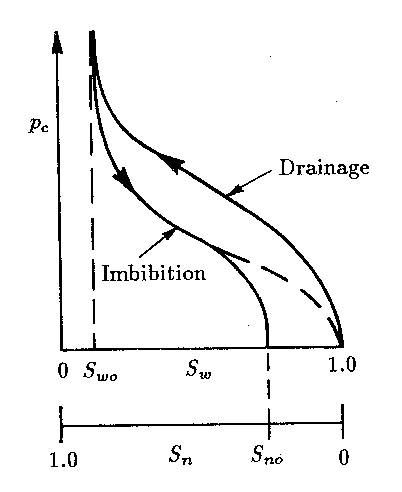
\includegraphics[width=0.43\columnwidth]{figures/HYSTER.EPS}
\caption{Capillary hysteresis \cite{Bea:72}, with
$S_{w} = S^w$, $S_{w0} =
S_r^w$, $S_{n} = S^{nw}$,
$S_{n0} = S_r^{nw}$ } 
\label{fig:hysteresis}
\end{center}
\end{figure}
%
\index{process - hysteresis capillary}

The capillary pressure/saturation relationships
differ for drainage and rewetting (imbibition) \cite{Mua:76}. This phenomenon is
called hysteresis (Fig. \ref{fig:hysteresis}). Reasons for capillary pressure hysteresis are:
(i) varying pore shape (ink-bottle effect), (ii) contact angle
hysteresis (raindrop effect), (iii) entrapment of non-wetting
fluids, (iv) swelling and shrinking of solid grains.

To introduce the concept of relative permeability we recall the
Darcy law for flow of multiple fluid phases through porous
media, equation (\ref{eqn:momentum_balance_fluid}).
Fig. \ref{fig:k_rel} shows an example of relative permeabilities for both wetting and non-wetting phases.

\begin{figure}[htb!]
\begin{center}
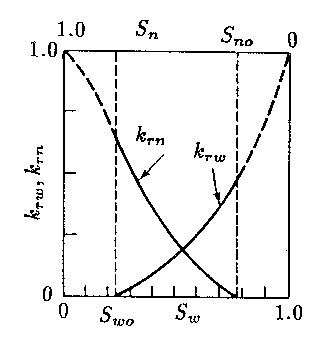
\includegraphics[width=0.45\columnwidth]{figures/K_REL.EPS}
\caption{Relative permeability functions \cite{Bea:72} with
$S_{w} = S^w$, $S_{w0} =
S_r^w$, $S_{n} = S^{nw}$,
$S_{n0} = S_r^{nw}$, $k_{rn} = k^{nw}$,
$k_{rw} = k^w$ } 
\label{fig:k_rel}
\end{center}
\end{figure}
%

We consider some of the most used models after van Genuchten, Haverkamp, Brooks-Corey.

%-------------------------------------------------------------------------------
\subsubsection*{van Genuchten model \cite{Van:80}}

The definitions of effective saturation, capillary pressure and relative permeability for the van Genuchten model are as follows
%
\begin{eqnarray}
S_{\mbox{\small eff}} = \frac{S^w - S_r^w}{1 -
S_r^w} = \left( 1 + (\alpha \, p_c)^n
\right)^m \qquad , \qquad p_c > 0
\end{eqnarray}
%
\begin{eqnarray}
p_c = \left\{
\begin{array}{ll}
0 & S^w >
S^w_{\mbox{\footnotesize max}}
\\
\frac{\rho^w g}{\alpha} (S_{\mbox{eff}}^{-1/m}-1)^{1/n} &
S_r^w < S^w <
S^w_{\mbox{\footnotesize max}}
\\
{p_c}_{\mbox{\footnotesize max}} & S^w <
S_r^w
\end{array}
\right.
\end{eqnarray}
%
with
\begin{eqnarray}
m = 1 - \frac{1}{n}
\end{eqnarray}
%
\begin{eqnarray}
\mathbf{k}_{\mbox{\small rel}}(h) 
= 
\frac{1-(\alpha h)^{n-2}\,[1+(\alpha h)^n]^{-m}}{[1+(\alpha h)^n]^{2m}}
\end{eqnarray}

Figs. \ref{fig:VanGenuhetenParameter} and \ref{fig:vG_krel} show the capillary pressure and relative permeability functions corresponding to the parameters given in Tab. \ref{tab:van_Genuchten}, respectively.

\begin{figure}[htb!]
\begin{center}
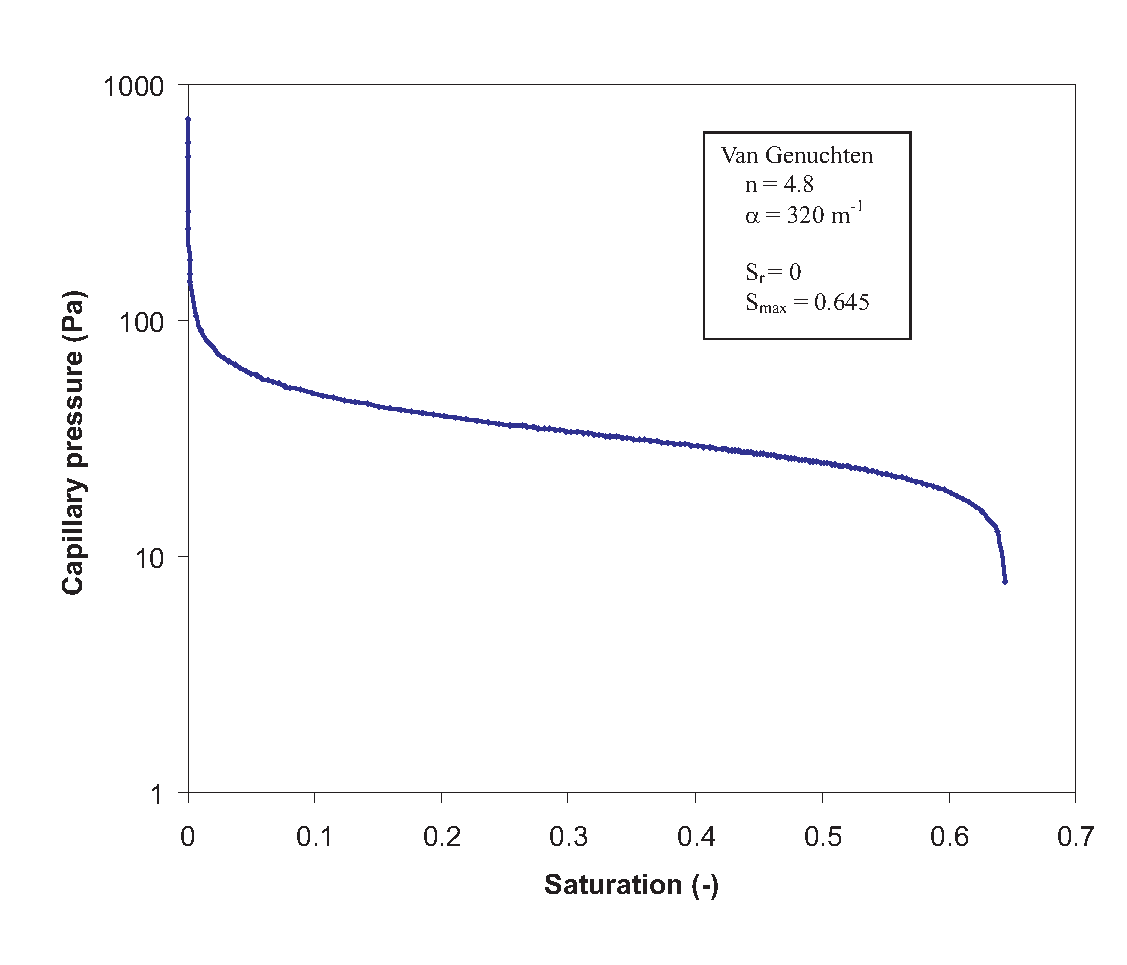
\includegraphics[width=0.7\columnwidth]{figures/VanGenuheten_P.eps}
\caption{Capillary pressure / saturation relationship (Tuebingen experiment
2005)} \label{fig:VanGenuhetenParameter}
\end{center}
\end{figure}
%

\begin{figure}[htb!]
\begin{center}
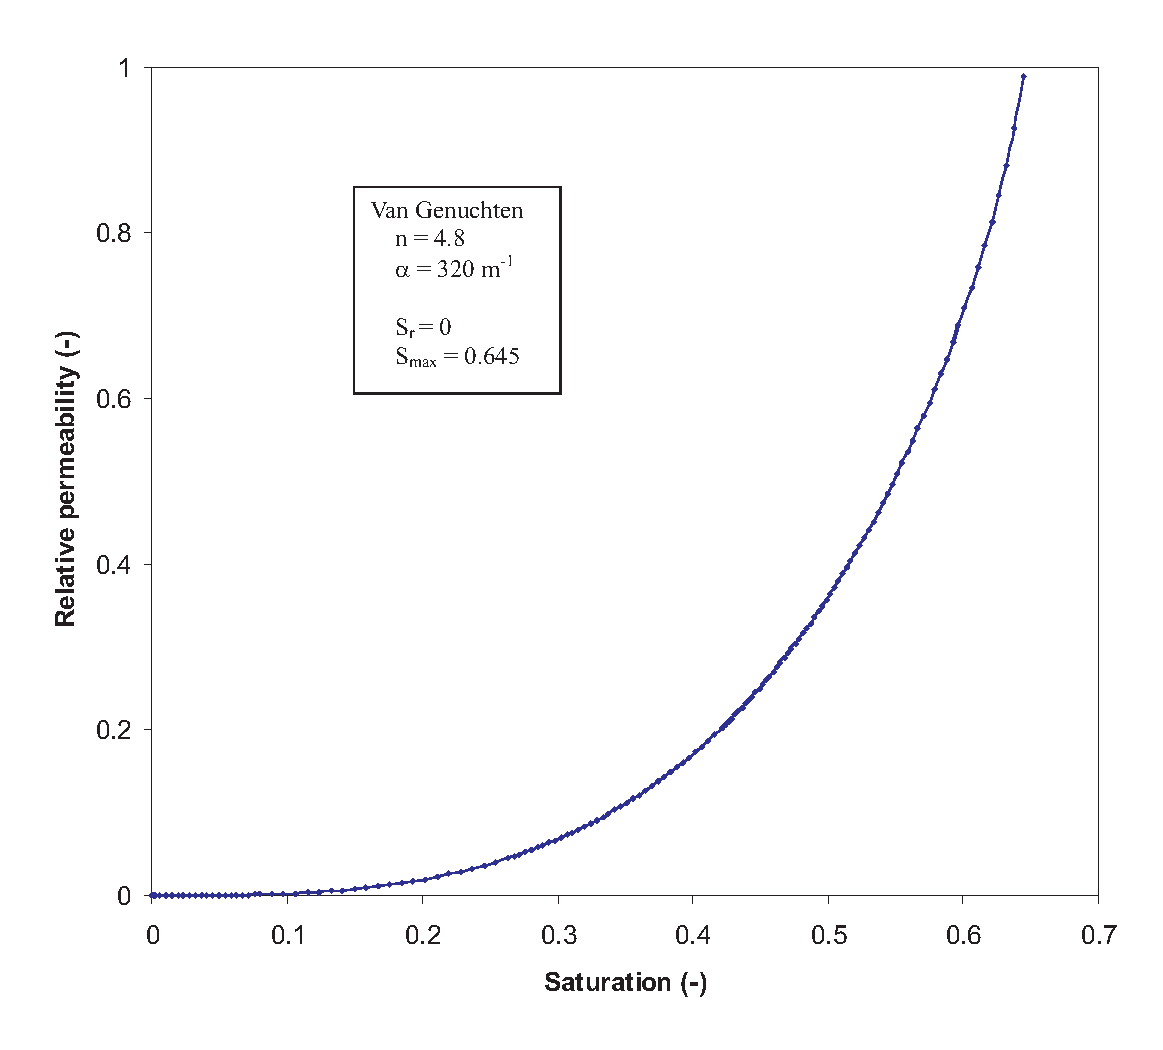
\includegraphics[width=0.6\columnwidth]{figures/VanGenuheten_K.eps}
\caption{Relative permeability / saturation relationship (Tuebingen experiment
2005)} 
\label{fig:vG_krel}
\end{center}
\end{figure}

% Tabelle als Gleitumgebung
\begin{table}[htb!]
\caption{Model parameter}
\label{tab:van_Genuchten}
\begin{center}
\begin{tabular}{|l|l|l|l|}
\hline
$S_r^w$     & residual water saturation &  $ 0 $   &   \\
$S^w_{max}$ & maximal water saturation   & $0.645$ & $$ \\
$n$         & vG parameter  & $4.8$ &  \\
$\alpha$    & vG coefficient  & $320$ & $[m^{-1}]$ \\
\hline
\end{tabular}
\end{center}
\end{table}
%

%-------------------------------------------------------------------------------
\subsubsection*{Haverkamp model \cite{HavVauTouWieVac:77}}

The formulas for the Haverkamp model are given in terms of pressure head
$h=p^w/g\rho^w$\index{quantity - pressure head}
and moisture content
$\theta=nS^w$.\index{quantity - moisture content}
%
The definitions of effective saturation, capillary pressure and relative permeability for the Haverkamp model are as follows
%
\begin{eqnarray}
\theta = \frac{\alpha(\theta_s-\theta_r)}{\alpha+|h|^\beta} +
\theta_r
\end{eqnarray}
\begin{eqnarray}
h = \left( -\frac{\alpha}{\theta} (\theta - \theta_s + \theta_r)
\right)^{1/\beta}
\end{eqnarray}
%
\begin{eqnarray}
\mathbf{k}_{\mbox{\small rel}}(h) = K_s \frac{A}{A+|h|^\beta}
\end{eqnarray}

%
% Tabelle als Gleitumgebung
\begin{table}[htb!]
\caption{Model parameter}
\label{tab:Haverkamp}
\begin{center}
\begin{tabular}{|l|l|l|l|}
\hline
$\theta$    & volumetric water (moisture) content &         & $[cm^3/cm^3]$ \\
$\theta_r$  & residual volumetric water content   & $0.075$ & $[cm^3/cm^3]$ \\
$\theta_s$  & saturated volumetric water content  & $0.287$ & $[cm^3/cm^3]$ \\
$h(\theta)$ & soil water pressure head            &         & $[cm]$ \\
            & relative to the atmosphere          &         & \\
$\alpha$    &                                     & $1.611\times 10^6$ & $[Pa^{-1}]$ \\
$\beta$     &                                     & $3.96$ & \\
\hline
\end{tabular}
\end{center}
\end{table}
%

Fig. \ref{fig:Haverkamp} shows the capillary pressure saturation function corresponding to the parameters given in Tab. \ref{tab:Haverkamp}.

% *** EPS-Grafik ***
\begin{figure}[htb!]
\begin{center}
\footnotesize
%\psfrag{Synonym}[pos][pos]{Tex-Ersetzung}
%\psfrag{x}[][]{$t$}
%\psfrag{y}[b][t]{$y(t)$}
%\psfrag{t}[][]{ }
\includegraphics[width=0.95\columnwidth]{figures/haver1.eps}
\caption{Hydraulic properties of unsaturated soil
\cite{HavVauTouWieVac:77}} 
\label{fig:Haverkamp}
\end{center}
\end{figure}
%

%-------------------------------------------------------------------------------
\subsubsection*{Brooks \& Corey model \cite{BroCor:64}}

The Brooks-Corey equations relating the saturation to the capillary pressure are
\begin{equation}
p^c\,=\,p^D\,S_{\mathrm{eff}}^{-(1/\lambda)}
\qquad\mbox{for}\qquad p^c\geq p^D
\label{eq29}
\end{equation}
%\begin{equation}
%S_{\mathrm{eff}}\,=\,
%\left\{
%\begin{array}{ccl}
%1                                                            & , & \quad p^c\leq p^D \\[2.0ex]
%\left(\frac{\textstyle{p^D}}{\textstyle{p^c}}\right)^\lambda & , & \quad p^c > p^D
%\end{array}
%\right.
%\label{eq29}
%\end{equation}
where $p^D$ is usually known as entry pressure, $\lambda$ is a pore-size distribution index.
%
$S_{\mathrm{eff}}$ is a normalized wetting fluid saturation. For the case of \co2 as wetting fluid into a saline aquifer it is defined as
\begin{equation}
S_{\mathrm{eff}}=\frac{S^{l}-S^l_{\mathrm{res}}}{1-S^l_{\mathrm{res}}-S^{CO_2}_{\mathrm{res}}} \\
\label{eq30}
\end{equation}
where $S^l_{\mathrm{res}}$ is the wetting phase residual or irreducible saturation, and $S^{CO_2}_{\mathrm{res}}$ is the nonwetting phase residual saturation. The constitutive parameters $p^D$, $\lambda$, $S^l_{\mathrm{res}}$ and $S^{CO_2}_{\mathrm{res}}$ are identified by fitting Eq.~(\ref{eq29}) to experimental data. Within this context, the entry pressure is to be understood as the minimum pressure that the nonwetting fluid must have to enter the largest pores. The relations between the relative permeability and the saturation are given by
\begin{eqnarray}
k_{\mathrm{rel}}^{l} & = & \left(S_{\mathrm{eff}}\right)^{(2+3\lambda)/\lambda}
\label{eq31} \\[2.0ex]
k_{\mathrm{rel}}^{CO_2} & = & \left(1-S_{\mathrm{eff}}\right)^2\,\left(1-\left(S_{\mathrm{eff}}\right)^{(2+\lambda)/\lambda}\right)
\label{eq32}
\end{eqnarray}


